% !TeX spellcheck = en_GB
% !TeX root = ../../build/architecture.tex

\section{Introduction}

\begin{frame}[allowframebreaks]{First Example: The Fibonacci State Machine}

\begin{columns}
\begin{column}{0.3\textwidth}
\begin{figure}
	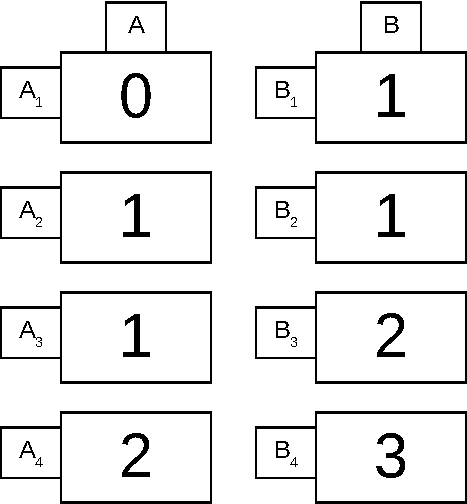
\includegraphics[width=\textwidth]{\zkevmdir/architecture/figures/fibonacci-sequence}
\end{figure}
\end{column}
%\hspace{-1.4cm}
\begin{column}{0.7\textwidth}
\begin{itemize}
\item We can build the Fibonacci state machine with two registries, $A$ and $B$.
\item In the Fibonacci sequence, we have the following relations between the states of these registries:
\begin{align*}
A_{i+1} &= B_i, \\
B_{i+1} &= A_i + B_i.
\end{align*}

\item Let's represent the states of these registries for four steps as polynomials in $\ZZ_p[x]$ evaluated 
on the group $H = \{\omega, \omega^2, \omega^3, \omega^4 = 1\}$:
\begin{align*}
A(\omega^i) &= A_i \quad \Longrightarrow \quad A = [0, 1, 1, 2] \\
B(\omega^i) &= B_i \quad \Longrightarrow \quad B = [1, 1, 2, 3]
\end{align*}
\end{itemize}
\end{column}
\end{columns}


%% ii
\begin{columns}
\begin{column}{0.3\textwidth}
\begin{figure}
	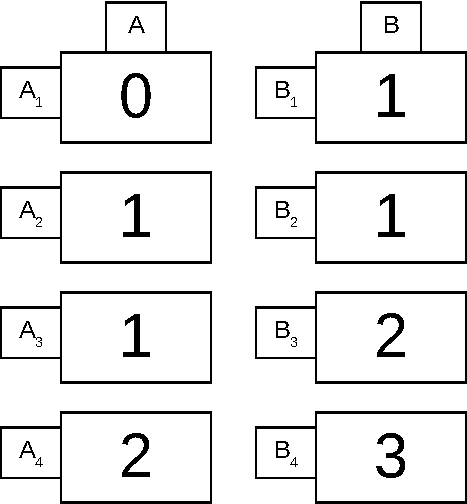
\includegraphics[width=\textwidth]{\zkevmdir/architecture/figures/fibonacci-sequence}
\end{figure}
\end{column}
%\hspace{-1.4cm}
\begin{column}{0.7\textwidth}
\begin{itemize}
\item The relations between the states of registries:
\begin{align*}
A_{i+1} &= B_i, \\
B_{i+1} &= A_i + B_i,
\end{align*}
for $i \in [4]$.
\item Are translated into relations (A.K.A identities) in the polynomial setting:
\begin{align*}
A(x\omega) &= \bigg\lvert_H  B(x), \\
B(x\omega) &= \bigg\lvert_H  A(x) + B(x).
\end{align*}
\end{itemize}
\end{column}
\end{columns}


%% iii
\begin{columns}
\begin{column}{0.3\textwidth}
\begin{figure}
	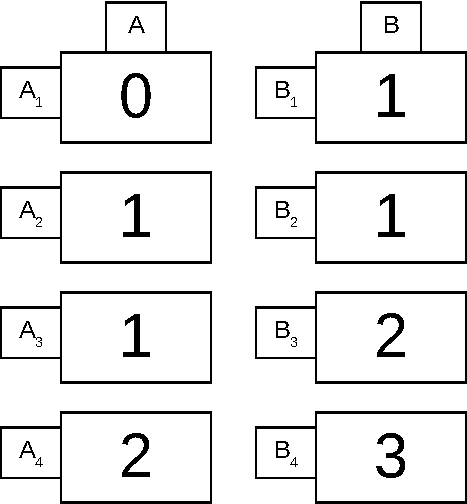
\includegraphics[width=\textwidth]{\zkevmdir/architecture/figures/fibonacci-sequence}
\end{figure}
\end{column}
%\hspace{-1.4cm}
\begin{column}{0.7\textwidth}

\begin{itemize}
\item So we have:

\vspace{-0.8cm}
\begin{align*}
A(x\omega) = \bigg\lvert_H  B(x), \quad
B(x\omega) = \bigg\lvert_H  A(x) + B(x).
\end{align*}
\item However, the previous identities do not correctly and uniquely describe our sequence because:
\begin{enumerate}
\item When we evaluate the identities in $\omega^4$:
\begin{align*}
A(\omega^5) = A(\omega) = 0 &\neq  3 = B(\omega^4), \\
B(\omega^5) = B(\omega) = 1 &\neq  5 = A(\omega^4) + B(\omega^4).
\end{align*}

The equations are not cyclic.
\item Other initial conditions also fulfill the identities, e.g:
$(2,3),(3,5),(5,8),(8,13)$.
\end{enumerate}
\end{itemize}
\end{column}
\end{columns}



%% iv
\begin{columns}
\begin{column}{0.4\textwidth}
\begin{figure}
	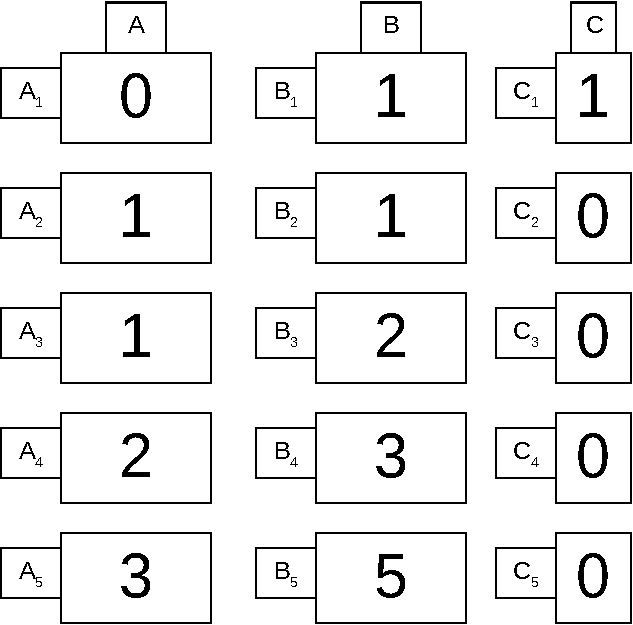
\includegraphics[width=\textwidth]{\zkevmdir/architecture/figures/fibonacci-sequence-aux}
\end{figure}
\end{column}
%\hspace{-1.4cm}
\begin{column}{0.6\textwidth}
\begin{itemize}
\item Let's add an auxiliary registry $C$ to solve these problems.
\item The corresponding polynomial is:
\begin{align*}
C(\omega^i) &= C_i \quad \Longrightarrow \quad C = [1, 0, 0, 0].
\end{align*}
\item With this auxiliary registry, we can now fix the polynomial identities as follows:
\begin{align*}
A(x\omega) &= \bigg\lvert_H  B(x)(1 - C(x\omega)), \\
B(x\omega) &= \bigg\lvert_H (A(x) + B(x))(1 - C(x\omega)) + C(x\omega).
\end{align*}
%\begin{align*}
%C(x)A(x) &= 0, \\
%C(x)(B(x) - 1) &= 0, \\
%A(x\omega) &=  B(x), \\
%B(x\omega) &=  A(x) + B(x).
%\end{align*}
\end{itemize}
\end{column}
\end{columns}


%% v
\begin{columns}
\begin{column}{0.4\textwidth}
\begin{figure}
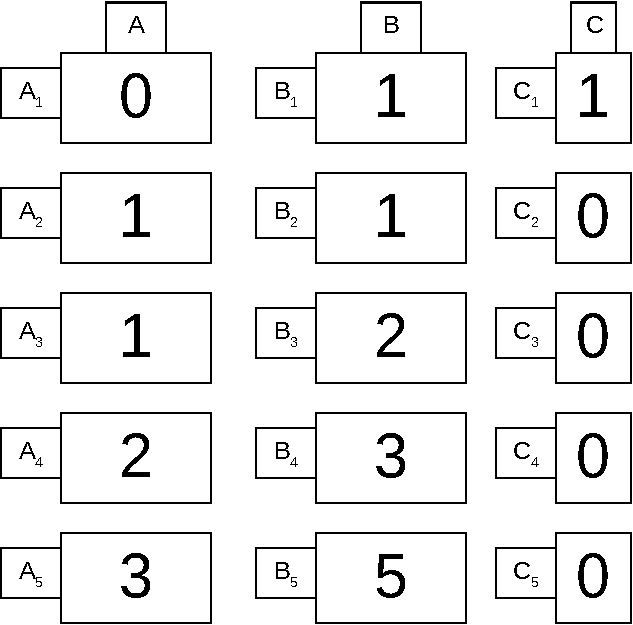
\includegraphics[width=\textwidth]{\zkevmdir/architecture/figures/fibonacci-sequence-aux}
\end{figure}
$C(x)$ is publicly known (A.K.A \textbf{pre-processed} or \textbf{constant}).
\end{column}

\begin{column}{0.6\textwidth}
\begin{itemize}
\item Note that now at $x = w^4$ the identities are satisfied:
\begin{align*}
A(x\omega) &= \bigg\lvert_H  B(x)(1 - C(x\omega)), \\
B(x\omega) &= \bigg\lvert_H (A(x) + B(x))(1 - C(x\omega)) + C(x\omega).\\
A(\omega^4 \omega) &= A(\omega^5) = A(\omega) = 0, \\
B(\omega^4 \omega) &= B(\omega^5) = B(\omega) = 1.
\end{align*}
\item We can also use other initial conditions $(A_0, B_0)$:
\begin{align*}
A(x\omega) &= \bigg\lvert_H  B(x)(1 - C(x\omega))+ A_0C(x\omega), \\
B(x\omega) &= \bigg\lvert_H  (A(x) + B(x))(1 - C(x\omega)) + B_0 C(x\omega).
\end{align*}
\end{itemize}
\end{column}
\end{columns}
\end{frame}





\begin{frame}[allowframebreaks]{Proving our State Machine (High Level)}
\begin{align*}
p_1(x)&= A(x\omega) - B(x)(1 - C(x\omega)) - A_0C(x\omega) = \bigg\lvert_H 0,\\
p_2(x) &= B(x\omega) - (A(x) + B(x))(1 - C(x\omega)) - B_0 C(x\omega) = \bigg\lvert_H 0.
\end{align*}

\begin{itemize}
\item We are going to convert these H-ranged identities into an $\FF$-ranged identities that 
is valid for any $x \in \FF$.
\item To do so, we are going to use the \textbf{zero polynomial} $Z_H(x)$.
\item $Z_H(x)$ is computed as the polynomial that is zero in $H$:
\[
(\omega,0), (\omega^2,0), (\omega^3,0), (\omega^4,0) \quad \Longrightarrow \quad Z_H(x) = (x-\omega)(x-\omega^2)(x-\omega^3)(x-\omega^4) = x^4-1.
\]
\item Notice that $p_1(x)$ and $p_2(x)$ have roots at $H$.
\item That means $Z_H(x) | p_1(x)$ and $Z_H(x) | p_2(x)$ 
because $(x-\omega)$, $(x-\omega^2)$, etc. are monomials of $p_1(x)$ and  $p_2(x)$.
\item Now we can compute $d_1(x) = p_1(x) / Z_H(x)$ and $d_2(x) = p_2(x) / Z_H(x)$.
\item The identities that need to be checked are $p_1(x) - d_1(x)Z_H(x) = 0$ and $p_2(x) - d_2(x)Z_H(x) = 0$ 
for any $x \in \FF$.

\vspace{0.15cm}
\begin{figure}
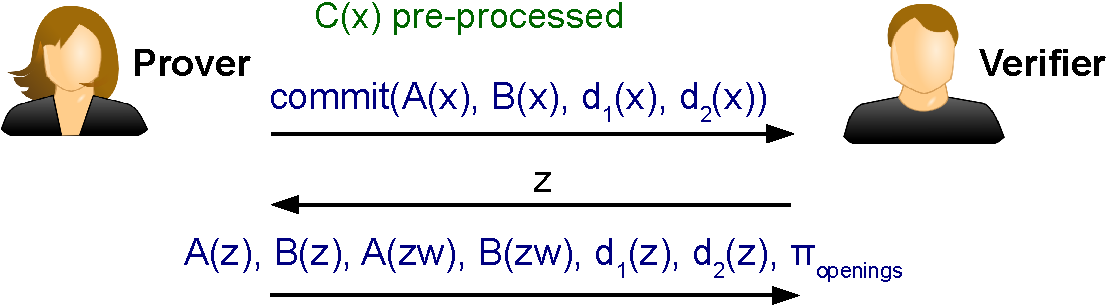
\includegraphics[width=0.65\columnwidth]{\zkevmdir/architecture/figures/proving-fibonacci}
\end{figure}
\end{itemize}
\end{frame}
